\documentclass[12pt]{article}

\usepackage{CJKutf8}
% 打中文時請務必加這個Package

\usepackage{epsfig,amsmath,amssymb,latexsym}
\usepackage{graphicx,epsfig,color,epsf,psfrag,hhline,amsmath,amssymb,textcomp}
%\usepackage{hyperref}
\usepackage{enumitem}

\setlength {\topmargin}{-1.0in}
\setlength {\textheight}{10in}
\setlength {\oddsidemargin}{-0.25in}
\setlength {\evensidemargin}{-0.25in}
\setlength {\textwidth}{6.75in}
\setlength {\parskip}{8pt plus 2pt minus 1pt}

\newtheorem{theorem}{Theorem}[section]
\newtheorem{definition}{Definition}[section]
\newtheorem{lemma}{Lemma}[section]

\newcommand{\comb}[2]{\left (\begin{array}{c} #1 \\ #2 \end{array} \right )}

\newcommand{\inlinecomb}[2]{\mbox{\scriptsize $\left (\begin{array}{c} #1 \\ #2 \end{array} \right )$\normalsize}}

\newcommand {\bsolution}{\noindent {\em Solution:} \ }

\newcommand{\esolution}{\hfill $\Diamond$ \\ \vspace{.3cm}}

%************************** Figure**********************************
\newcommand {\bfig}[2] {\begin{figure}[htbp]
                        \centerline {
                         \epsfig{figure={#1},clip=,width={#2}}}}

\newcommand {\efig}[2]{ \caption{#2}
                        \label{fig:#1}
                        \end{figure}
                        \mymarginpar{fig:#1}}
\newcommand {\rfig}[1]{Figure \ref{fig:#1}}

%%%%%%%%%%%%%%%%%%%%%%%%%%%%%%%%%%%%%%%%%%%%%%%%%

\begin{document}
\thispagestyle{empty}
\begin{center}
{\Large \noindent COM 530500 {\bf Network Science Homework \#3} \\
\large {{\sc Due:} Thursday, December 23, 2021}  \\
}
\emph{No late homework will be accepted}.
\end{center}


\noindent {\begin{CJK}{UTF8}{bsmi}
{\bf 班級:} 資應所
\end{CJK}}

\noindent  {\begin{CJK}{UTF8}{bsmi}
{\bf 姓名:} 鄭程哲
\end{CJK}}

\noindent {\begin{CJK}{UTF8}{bsmi}
{\bf 學號:} 110065512
\end{CJK}}

\bigskip

%---------------------------------------------------------------------------
% Problem 1
%---------------------------------------------------------------------------

\noindent {\bf Problem 1. (40\%)} One can calculate the diameter of certain types of networks exactly:
\begin{enumerate}[label=(\alph*)]
	\item (10\%) What is the diameter of a clique?
	\item (10\%) What is the diameter of a square portion of square lattice, with $L$ edges (or equivalently $L+1$ vertices) along each side, like figure \ref{square_lattice}.
	\begin{figure}[h]
		\centering
		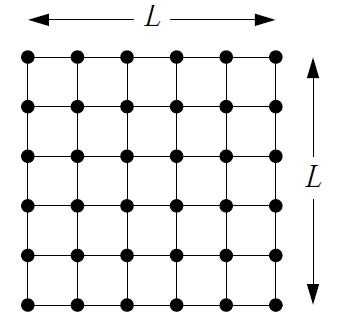
\includegraphics[width=0.45\textwidth]{NS_HW_Fig_1.jpg}
		\caption{Square lattice}
		\label{square_lattice}
	\end{figure}
	\item (10\%+10\%) A Cayley tree is a symmetric regular tree in which each vertex is connected to the same number $k$ of others, until we get out to the leaves, like figure \ref{Cayley_tree} (We have $k = 3$ in figure \ref{Cayley_tree}). Show that the number of vertices reachable in $\ell$ steps from the central vertex is $k(k-1)^{\ell-1}$. ({\it Hint: by induction}) Hence find an expression for the diameter of the network in terms of $k$ and the number of vertices $n$.
	\begin{figure}[h]
		\centering
		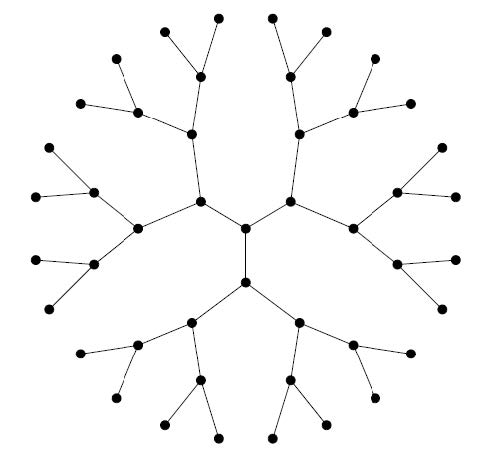
\includegraphics[width=0.45\textwidth]{NS_HW_Fig_2.jpg}
		\caption{Cayley tree with $k = 3$}
		\label{Cayley_tree}
	\end{figure}
\end{enumerate}

\bsolution
%---------------------------------------------------------------------------
\begin{enumerate}[label=(\alph*)]
	\item  A clique is an undirected network such that every node is connected by and edge to every other. Therefore, the length of geodesic path of any pair of nodes is 1. The diameter of a clique is 1.
	\item The longest geodesic distance, i.e. diameter, occurs at the nodes on the diagonal, which is $2L$.
	\item Prove by induction: \\
			When $l=1, k(k-1)^{l-1}=k(k-1)^0=k$ is true. \\
			Assume that when $l=n, k(k-1)^{n-1}$ is true. There are $k(k-1)^{n-1}$ leaves, and each leaf would generate $k-1$ leaves because one edge is connected to its parent. \\
			When $l=n+1$, the number of verteices reachable is $k(k-1)^{n-1}*(k-1)=k(k-1)^{(n+1)-1}$. The inductive step also holds true. Since both the base case and the inductive step have been proved as true, by mathematical induction the statement $k(k-1)^{l-1}$ holds for every natural number $l$. \\\\
		The longest geodesic distance is one of the paths from leaf to leaf. Suppose that $L$ means the steps from root to leaf, the diameter is therefore equal to $2L$. Our goal is to solve $L$.\\
		\begin{align*}
			1+\sum_{l=1}^{L}{k(k-1)^{l-1}} &= n \\
			\sum_{l=1}^{L}{k(k-1)^{l-1}} &= n-1 \\
			\frac{k(1-(k-1)^L)}{1-(k-1)} &= n-1 \\
			1-\frac{(n-1)(2-k)}{k} &= (k-1)^L \\
			\frac{\log{(1-\frac{(n-1)(2-k)}{k})}}{\log{(k-1)}} &= L
		\end{align*}
		Hence, the diameter is
		\begin{align*}
			2L &= 2\frac{\log{(1-\frac{(n-1)(2-k)}{k})}}{\log{(k-1)}}
		\end{align*}
\end{enumerate}
%---------------------------------------------------------------------------
\esolution

\newpage
%---------------------------------------------------------------------------
% Problem 2
%---------------------------------------------------------------------------

\noindent {\bf Problem 2. (45\%)} Consider the random graph $G(n,p)$ with mean degree $c$.\\
\begin{enumerate}[label=(\alph*)]
	\item (15\%) Show that in the limit of large $n$ the expected number of triangles in the network is $\frac{1}{6}c^3$.
	\item (15\%) Show the expected number of connected triples in the network is $\frac{1}{2}nc^2$ for $n$ large.
	\item (15\%) Show the clustering coefficient $C$ goes to $0$ when $n$ goes to infinity.
	
\end{enumerate}

\bsolution
%---------------------------------------------------------------------------
\begin{enumerate}[label=(\alph*)]
	\item Triangle means there is a edge between any 2 vertices in any 3 vertices combination. In random graph $G(n, p), p$ is the probability that there is a edge between any distinct pair. We have that
		\begin{align*}
			p = \frac{c}{n-1}\text{.}
		\end{align*}
	So, the expected number of triangles in the network is
		\begin{align*}
			\lim_{n \to \infty}{n \choose 3}p^3 = \lim_{n \to \infty}\frac{n(n-1)(n-2)}{6}\frac{c^3}{(n-1)^3}=\frac{1}{6}c^3\text{.}
		\end{align*}
	\item Connected triple means there are 2 vertices connected to an anchor vertex. Firstly pick an anchor vertex and two other vertices. Then connect these two vertices with the anchor vertex. So, the expected number of connected triples in the network is as follows.
		\begin{align*}
			\lim_{n \to \infty}{n \choose 1}{n \choose 2}p^2=\lim_{n \to \infty}\frac{n}{1}\frac{n(n-1)}{2}\frac{c^2}{(n-1)^2}=\frac{1}{2}nc^2
		\end{align*} 
	\item Clustering coefficient can be calculated by the formula below.
		\begin{align*}
			C &= \frac{(\text{\# of triangles})*3}{(\text{\# of connected triples})} \\
			C &= (\frac{1}{6}c^3*3) / (\frac{1}{2}nc^2)=\frac{c}{n}
		\end{align*}
		The clustering coefficient $C$ goes to 0 when $n$ goes to infinity.
\end{enumerate}
%---------------------------------------------------------------------------
\esolution

%---------------------------------------------------------------------------
% Problem 3
%---------------------------------------------------------------------------
\noindent {\bf Problem 3. (15\%)} Consider the example model discussed in Section 13.8.1 in \cite{newman2010networks}, a configuration model with vertices of degree three and less only and generating functions given by $g_0(z) = p_0 +p_1z +p_2z^2 +p_3z^3$, and $g_1(z) =\frac{g_0^{\prime}(z)}{g_0^{\prime}(1)} = q_0 +q_1z +q_2z^2$. In the regime in which there is no giant component, show that the average size of the component to which a randomly chosen vertex belongs is $$\langle s \rangle=1+\frac{(p_1+2p_2+3p_3)^2}{p_1-3p_3}\text{.}$$

\newpage
\bsolution
%---------------------------------------------------------------------------
We have that

	$$g_1(z)=\frac{g'_0(z)}{g'_0(1)}=\frac{p_1+2p_2z+3p_3z^2}{p_1+2p_2+3p_3}=q_0+q_1z+q_2z^2,$$
	$$\text{where }q_0=\frac{p_1}{p_1+2p_2+3p_3}, q_1=\frac{2p_2}{p_1+2p_2+3p_3}, q_2=\frac{3p_3}{p_1+2p_2+3p_3} \text{.}$$

	$$ \langle s \rangle=\frac{\sum s\pi_s}{\sum \pi_s}=\frac{h'_0(1)}{g_0(u)}$$
	$$ \because h'_0(z)=\frac{h_0(z)}{z}+g'_0(1)h_1(z)h'1(z) $$
	$$ h'_0(1)=g_0(u)+g'_0(1)uh'_1(1) $$
	$$ h'_1(z)=\frac{h_1(z)/z}{1-zg'_1(h_1(z))} $$
	$$ h'_1(1)=\frac{u}{1-g'_1(u)} $$
	$$ \therefore\langle s \rangle=1+\frac{g'_0(1)u^2}{g_0(u)(1-g'_1(u))} $$
	When there is no giant component, $S=0$ and $u=1$. $g'_0(1)=p_1+2p_2+3p_3$ and $g'_1(1)=q_1+2q_2$.\\
	Therefore, $$ \langle s \rangle=1+\frac{g'_0(1)}{1-g'_1(1)}=1+\frac{p_1+2p_2+3p_3}{1-q_1-2q_2}\text{.}$$
	$$ \langle s \rangle=1+\frac{p_1+2p_2+3p_3}{\frac{p_1-3p_3}{p_1+2p_2+3p_3}}=1+\frac{(p_1+2p_2+3p_3)^2}{p_1-3p_3} $$
	
%---------------------------------------------------------------------------
\esolution

%---------------------------------------------------------------------------
% The end of problems.
%---------------------------------------------------------------------------

%---------------------------------------------------------------------------
% References
%---------------------------------------------------------------------------
\begin{thebibliography}{9}
\bibitem{newman2010networks} Newman, Mark. \emph{Networks: An Introduction.} Oxford University Press, 2010.
\end{thebibliography}

\end{document}
